%% We use `subfiles' package
\documentclass[preamble.tex]{subfiles}
\begin{document}

\clearpage

\chapter{Nested Data Parallelism}

In this chapter I will introduce the reader to the context of my work - the \name{Data Parallel Haskell} (\DPH) project\idph{}.

\DPH has very specific requirements for the fusion system to satisfy in order to be effective. While the fusion concepts I discuss in later chapters are widely applicable to areas of high performance computing beyond nested data parallelism, it did have a heavy influence on the fusion system I have developed.


\section{Data Parallel Haskell}
\label{sec:DPH}

\name{Data Parallel Haskell (DPH)}\idph{} is a library for and an extension to the \Haskell programming language, providing high level access to \*nested data parallelism*.

\term{Nested data parallelism}\idx{data parallelism: nested}{} is a type of \name{SPMD}\idx{data parallelism: SPMD (single program, multiple data)}{} parallelism (single program, multiple data) which operates on \*irregular*\idx{data structure: irregular} data structures. Two examples of irregular data structures are \*sparse matrices*\idx{data structure: sparse matrix} and \*unbalanced trees*\idx{data structure: unbalanced tree}.

In a nested data parallel program, parallel computations can call further data parallel computations. For example when traversing an unbalanced tree each node may process each of its children in parallel. Without statically knowing the branching of the tree, it may be difficult to adequately parallelise the process. \DPH offers an elegant solution through its vectorisation process which will be discussed in Section \ref{sec:Vectorisation}.

\DPH takes an active part in the optimisation and the compilation of its client code. It guides the compilation process in many ways including vectorisation \cite{PLKC08}, choosing the optimal data representation \cite{CDL09} as well as applying fusion \cite{CLP+07} and rewrite rules \cite{PTH01} to improve performance.

In essence \DPH reimplements the familiar list interface in terms of seamlessly parallelised arrays. Listing \ref{lst:DPH-interface} shows some of the most important functions in the \DPH interface. Since \DPH has language support, the bracket notation for parallel arrays closely resembles that for \Haskell lists: @[:a:]@ denotes a parallel array of type @a@, while @[:[:a:]:]@ is a nested parallel array. The counterpart of \Haskell's list comprehensions is also present and is called \*parallel array comprehensions*.


\begin{hscode2}[%
	caption={Type signatures for parallel array operations.},%
	label=lst:DPH-interface%
]
(!:)         :: [:a:] -> Int -> a
sliceP       :: [:a:] -> (Int,Int) -> [:a:]
replicateP   :: Int -> a -> [:a:]
mapP         :: (a -> b) -> [:a:] -> [:b:]
zipP         :: [:a:] -> [:b:] -> [:(a,b):]
zipWithP     :: (a -> b -> c) -> [:a:] -> [:b:] -> [:c:]
filterP      :: (a -> Bool) -> [:a:] -> [:a:]

concatP      :: [:[:a:]:] -> [:a:]
concatMapP   :: (a -> [:b:]) -> [:a:] -> [:b:]
unconcatMapP :: [:[:a:]:] -> [:b:] -> [:[:b:]:]
transposeP   :: [:[:a:]:] -> [:[:a:]:]
expandP      :: [:[:a:]:] -> [:b:] -> [:b:]

combineP     :: [:Bool:] -> [:a:] -> [:a:] -> [:a:]
splitP       :: [:Bool:] -> [:a:] -> ([:a:], [:a:])
\end{hscode2}



Collective operations on parallel arrays are executed in parallel when the hardware supports it. The framework is targeting shared memory architectures and uses \Haskell threads \cite{Jones08atutorial} to achieve parallelism.

By design the computation is split evenly across the available processing elements\footnote{\term{Processing element} is a general term referring to processors, processor cores or hardware threads.} which includes highly irregular parallel programs. The next sections will \todo{outline the library structure,} cover the basics of vectorisation and describe the current stages of fusion in \DPH.


\todo{\section{DPH structure}}

\clearpage

\section{Vectorisation}
\label{sec:Vectorisation}
\ivect{}

The principle idea behind \DPH was to allow the programmer write parallel programs without the additional effort of parallelising, scheduling, load balancing and low level optimisation.

The work on \DPH was originally inspired by Blelloch's pioneering work on \name{NESL} \cite{BCH+}, a research language designed to explore the new approach to nested data parallelism\idx{data parallelism: nested}{}.

At the core of \DPH is the vectoriser which is implemented in the \name{Glasgow Haskell Compiler}\footnote{Glasgow Haskell Compiler: http://www.haskell.org/ghc} (\GHC).

\begin{bluebox}
\name{Vectoriser} transforms \term{nested} data parallelism to \term{flat} data parallelism by means of \term{flattening transform} on \*data* and \term{lifting transform} on \*functions*.
\end{bluebox}

The two transforms are described in the following sections.



\subsection{Flattening transform}
\label{sec:Flattening}
\idx{flattening transform}{}


\begin{figure}
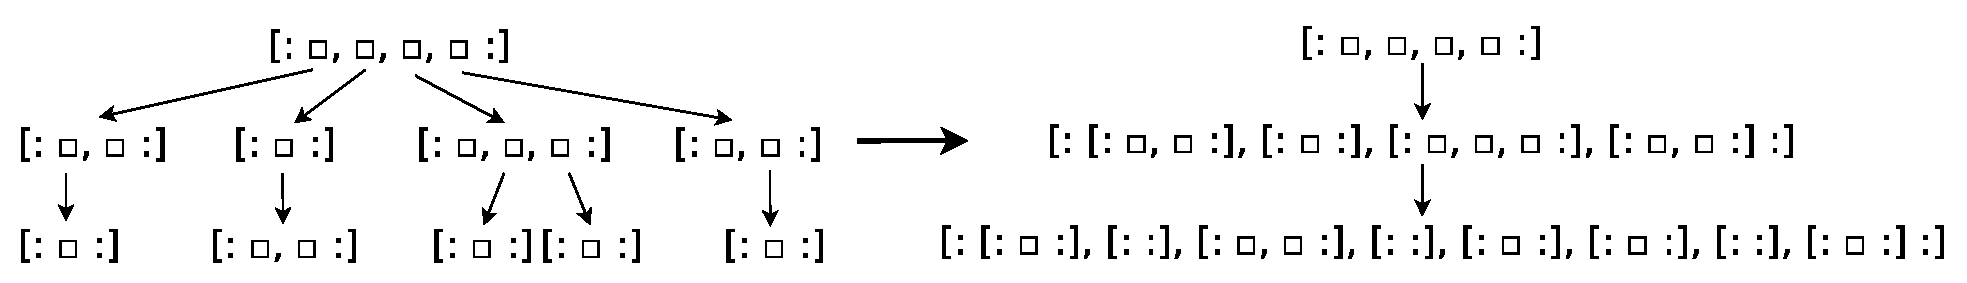
\includegraphics[width=1\textwidth]{img/TreeRepr}
\caption{Value of type \code{[:Tree:]} (left) and its flattened representation (right). Empty subtrees are omitted from the conceptual representation.%
\label{fig:TreeRepr}}
\end{figure}


Suppose we wanted to store trees of an arbitrary shape\idx{data structure: tree}{}. The following definition of a tree using parallel arrays is not unlike those a Haskell programmer would write using lists:

\begin{hscode}
data Tree = Tree Int [:Tree:]
\end{hscode}

A sample tree is given on the left of Figure \ref{fig:TreeRepr}. Just by looking at the top level of the tree it would not be possible to know what the branching is.

Now suppose we wanted to apply some function @f@ to every node of the tree:


\begin{hscode}
visit :: (Int -> Int) -> Tree -> Tree
visit f (Tree v children) = Tree (f v) children'
  where children' = mapP (visit f) children
\end{hscode}


Since the array of @children@ may be small, we are unlikely to gain any performance by parallelising the call to @mapP@. Additionally every @visit@ to a child node would potentially spawn more tiny parallel computations. 
% A naive tree representation would have probably failed to provide us with enough clues on how to split the load between processing elements.

\begin{bluebox}
The \term{flattening transform} translates \*nested data* in user programs to \*flat data representation*.
\end{bluebox}

The right of Figure \ref{fig:TreeRepr} shows the same tree with each of its levels placed into a \term{nested parallel array}\idx{nested: parallel array}{}.

At runtime a \*nested parallel array* (e.g. each level of a tree) is represented by a \term{data array} and a \term{segment descriptor}\isegd{}. The flat data array stores all the nodes' values, while the segment descriptor defines the partitioning to recreate the original nesting.

The following nested parallel array may have been the deepest level of the discussed tree:

\begin{hscode}
[: [:5:], [::], [:4,2:], [::], [:3:], [:17:], [::], [:11:] :]
\end{hscode}

At runtime it would be stored as an array of data values together with the segment descriptor containing the lengths and the starting index positions of the contained arrays (offsets into the data array)\footnote{Technically the array of index offsets can be computed from the array of lengths. It is stored with the segment descriptor for efficiency reasons.}:

\begin{hscode}
[# 5, 4, 2, 3, 17, 11 #]       -- data

[# 1, 0, 2, 0, 1, 1, 0, 1 #]   -- lengths
[# 0, 1, 1, 3, 3, 4, 5, 5 #]   -- indices
\end{hscode}

As a result every level of a tree can be efficiently processed in parallel.

In summary, flattening transform allows the user to define data which is then automatically aggregated into parallel arrays.

In the following section we discuss the lifting transform which vectorises the functions that can be applied to the flattened data.


\subsection{Lifting transform}
\label{sec:Lifting}

We have discussed the way the data is represented in \DPH but said nothing about how the vectoriser adapts the functions to fit the new data representation.

The lifting transform turns functions on values (@a@) into functions on arrays (@[:a:]@). Similarly, and functions on arrays (@[:a:]@) into functions on nested arrays (@[:[:a:]:]@).

It is not necessary to delve into too much detail here, since by the time the lifted code is compiled in backend of \DPH (where the fusion takes place) it is no longer a concern as to how it is done.

In order to illustrate the basics of the lifting transform we will use the following function as an example:

\begin{hscode}
f :: Float -> Float
f x = x * x + 1
\end{hscode}

For every such function the vectoriser generates its \*lifted* version @f^@ replacing all inner functions by their \*lifted* counterparts and all constants by calls to @replicateP@:

\begin{hscode}
f^ :: [:Float:] -> [:Float:]
f^ x = (x *^ x) +^ (replicateP n 1)
  where n = lengthP x
\end{hscode}

This new definition obeys the rule @f^ = mapP f@, thus it is possible to replace @(mapP f)@ with @f^@.

In the generated code\footnote{The code generated internally to be used with the backend library of array operations.} @f^@ becomes the following\footnote{This is no longer true for functions as simple as \code{f} \cite{vectavoid} but it is still a valid example indicative of \DPH inner workings }:

\begin{hscode}
f^ :: Array Float -> Array Float
f^ x = zipWith (+) (zipWith (*) x x)
                   (replicate n 1)
  where n = length x
\end{hscode}

The above code is an example of the code which is compiled against the backend library of flat array combinators. One will notice that this code would produce two intermediate arrays\iintermediate{}. \DPH relies on subsequent fusion optimisation to remove these intermediate results and compute @f^@ in one traversal of the input array.

% If we return to the original tree example from the previous section, there we may need to apply @f@ to an array of arrays. The flat data representation we chose allows us to easily derive @f^^@ in terms of @f^@ like this:

% \begin{hscode}
% f^^ :: [:[:Float:]:] -> [:[:Float:]:]
% f^^ xss = unconcatP xss (f^ (concatP xss))
% \end{hscode}

% Recalling that we use a flat data array together with a segment descriptor to represent @xss@, it becomes clear that both @concatP@ and @unconcatP@ are simple constant time operations that do nothing more than replacing one segment descriptor with another.

Vectorisation is more thoroughly covered in \cite{PLKC08}. However, since some of the code generated by the vectoriser is particularly idiomatic, I will come back to the topic of vectorisation at various points of this thesis.

\todo{Maybe talk about double-lifting something like @scanP 0 (\z xs -> mapP f x)@.}


\clearpage

\section{Data Representation}
\label{sec:DPH-Data-Representation}

\Haskell allows for a very high-level of expressiveness when it comes to user-defined types. \DPH attempts to support this expressiveness and allow the programmer to create and compose types to be used in \DPH programs. We have already an example of a recursive tree type in Section \ref{sec:Flattening} which is fully supported by \DPH.

Over the next several pages I will briefly outline how \DPH chooses the data representation.


\subsection{Unboxed values}
\iboxing{}

Regular \Haskell values, such as @Int@s and @Float@s are stored as boxed values on the heap. This means that an array of such values would be stored as array of pointers to the heap allocated values which would be a major hit on performance. It would incur boxing/unboxing costs as well as make it impossible to cache multiple consecutive elements at a time.

Instead, \DPH uses arrays of unboxed values in its backend which will be referred to as \*unboxed arrays*.


\subsection{Product types}

\Haskell's product types, or the tuples of two of more heterogeneous elements, are allocated as boxed values on the heap. As discussed, dereferencing heap allocated values considerably affects performance. Instead, an array of pairs @[:(a,b):]@ is stored as a pair of arrays @([:a:],[:b:])@. Similarly an array of larger n-tuples becomes an n-tuple of arrays.

This parametric representation is made possible through the use of type families as described in \cite{CDL09}.


\subsection{Sum types}

One distinctive feature of \DPH is that is allows one to use user defined data types. We have already seen how a user could define a data type for @Tree@. Likewise we could define a new data type @Shape@ with two constructors:

\begin{hscode}
data Shape = Circle Float
           | Rectangle Int Int
\end{hscode}

In \DPH the values constructed by the \*same constructor* are stored in the same array. To store an array @[:Shape:]@ the following arrays are used:
\begin{itemize}
\item An array @[:Float:]@ that stores radii of all circles
\item A pair of arrays @([:Int:],[:Int:])@ that sore dimensions of all rectangles
\item A \*selector*\idx{selector}{} array [:Int:] which determines which of the two constructors has been used. The selector array allows to recreate the original interleaving of values constructed with different constructors.
\end{itemize}

Having multiple arrays, each storing only the relevant values wrapped by the same constructor, not only avoids the cost of unboxing but also facilitates pattern matching on constructors.


\clearpage

\section{Backend and Fusion}

By the time the backend is reached in the compilation pipeline the nested data parallelism\idx{data parallelism: nested}{} in the original user program has been completely transformed to flat data parallelism:
\begin{itemize}
\item The program is now expressed in terms of flat and \*segmented array combinators*\isegmented{} that take the segment descriptor as an additional argument.\todo{Some of these segmented operations are shows in listing...}
\item All data is now represented in terms of flat unboxed\iboxing{} data arrays and segment descriptors\isegd{}.
\item As discussed in Section \ref{sec:DPH-Data-Representation} the vectoriser has also stripped out the product and sum types including those defined by the user and conveniently arranged them in flat arrays.
\end{itemize}

Thus the backend, or the library of array combinators\icomb{}, only needs to support the arrays of primitive types (@Int@, @Double@, @Bool@, etc. and tuples of these). This is where both the fusion and parallelisation occur.

% The backend library implements a fixed interface that is called by the vectoriser. The support for any architectures other than multi-core systems can be added through reimplementing the primitive library interface, though the parallel programming model heavily relies on shared memory architectures for efficiency. The primitive library in its current state uses the Vector library\footnote{http://hackage.haskell.org/package/vector } to store arrays and Haskell threads to implement parallelism \cite{Jones08atutorial}. Essentially each thread is given a chunk of array(s) and a sequential operation to apply to it.

\todo{Possibly kill everything below}

\DPH system originally introduced fusion at two levels:
\begin{description}
\label{list:DPH-fusion-levels}
\item \textbf{Removing synchronisation points}

Due to the use of \Haskell threads \cite{Jones08atutorial}, the code responsible for distributing the processing across the processing elements\ipe{} introduces many thread @fork/join@ points. This prohibits the application of array fusion that we discussed in the previous chapter. Thus if there is no processing to be done between the @join@ and the next @fork@, these are fused together using the rewrite rules\irwrules{} \cite{PTH01}.

\item \textbf{Stream Fusion}

When I started\name{Stream Fusion}\istreamfusion{} receives the most attention as far as the fusion in \DPH goes. It not only considerably affects the internal implementation of collective array operations in \DPH and in the underlying \name{Vector} library\footnote{http://hackage.haskell.org/package/vector}, but also relies on a certain set of optimisations in the compiler. A description of \name{Stream Fusion} is given in Appendix \ref{sec:Stream-Fusion}. Just like the fusion that removes superfluous synchronisation points, \name{Stream Fusion} also heavily relies on inlining and rewriting to work.
\end{description}

Unfortunately, the common point of failure of all of the above fusion types is that they rely on the consecutive operations being inlined and being adjacent to each other for the rewrite rules to fire. \todo{They are subject to the shortcomings of equational fusion systems I discussed in Section ref}

Over the following several chapters I will present my own replacement backend for \name{Data Parallel Haskell} which enables the fusion in more cases than was possible with previous fusion systems.


\IfNotCompilingAll{\bibliography{bib}}


\end{document}